\documentclass[tikz,border=6pt]{standalone}
\begin{document}
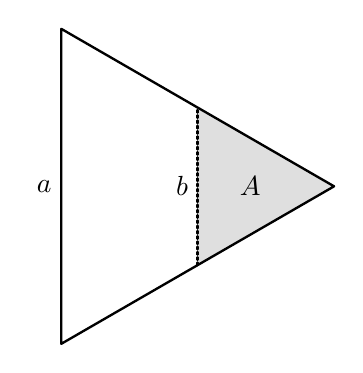
\begin{tikzpicture}[line cap=round,line join=round]
\fill[gray!25] ({2*sqrt(3)},0)--({sqrt(3)},1)--({sqrt(3)},-1)--cycle;
\draw[line width=.85pt] (0,-2)--(0,2)--({2*sqrt(3)},0)--cycle;
\draw[densely dotted,line width=.9pt] ({sqrt(3)},-1)--({sqrt(3)},1);
\node[left] at (0,0) {$a$};
\node[left] at ({sqrt(3)},0) {$b$};
\node at (2.4,0) {$A$};
\end{tikzpicture}
\end{document}
